%aom2018.tex
\documentclass[12pt,letterpaper]{article}
\usepackage{mathptmx}
\usepackage[margin=1in]{geometry}
\usepackage[titletoc,title]{appendix}
\usepackage{tabularx, longtable, pdflscape, rotating, adjustbox}  % for 'tabularx' environment and 'X' column type

\usepackage{ragged2e}  % for '\RaggedRight' macro (allows hyphenation)
\newcolumntype{Y}{>{\RaggedRight\arraybackslash}X} 
\usepackage{booktabs}  % for \toprule, \midrule, and \bottomrule macros 

\usepackage{setspace}
\doublespacing
  
\usepackage{amssymb,latexsym}
\usepackage[round,sort]{natbib}
\usepackage{fancyhdr}
\usepackage{lastpage}
\usepackage{graphicx,multirow}
\usepackage{titling}
\graphicspath{ {aom2018/} }

% Bold Table and Figure captions
\usepackage{caption}
\captionsetup{figurename=FIGURE}
\captionsetup{tablename=TABLE}
\captionsetup[figure]{labelfont=bf}
\captionsetup[table]{labelfont=bf}
  
% Turns off all section numbering
\setcounter{secnumdepth}{0} 
\usepackage{titling}
\usepackage[nolists]{endfloat}
\DeclareDelayedFloatFlavor{sidewaystable}{table}
\DeclareDelayedFloatFlavor{sidewaysfigure}{figure}

  % Places all tables at end of document and creates AOM-style table-here placeholders
  \usepackage[nolists]{endfloat} % Places all figures and charts at end of manuscript and adds 'insert table x about here' lines.
  \renewcommand{\figureplace}{
    \begin{center}
    \begin{singlespace}
    ------------------------------------\\
    Insert \figurename \ \thepostfig\ about here.\\
    ------------------------------------
    \end{singlespace}
    \end{center}}
  \renewcommand{\tableplace}{%
    \begin{center}
    \begin{singlespace}
    ------------------------------------\\
    Insert \tablename \ \theposttbl\ about here.\\
    ------------------------------------
    \end{singlespace}
    \end{center}}

  \usepackage{titlesec}
   \titleformat{\title}
       {\filcenter\normalfont\bfseries\uppercase}{\thetitle}{1em}{}
  \titleformat{\section}
    {\filcenter\normalfont\bfseries\uppercase}{\thesection}{1em}{}
  \titleformat{\subsection}
    {\normalfont\bfseries}{\thesubsection}{1em}{}
  \titleformat{\subsubsection}[runin]
   {\normalfont\bfseries\slshape}{\thesubsubsection}{1em}{\hspace*{\parindent}}
       
\usepackage{tabu}
\usepackage{textcomp}
\usepackage{listings}
\usepackage{hyperref}
\usepackage{verbatim}
\usepackage{tabu}
\hypersetup{
    colorlinks=true,
    linkcolor=blue,
    filecolor=cyan,      
    urlcolor=cyan,
    citecolor=blue,
}

\usepackage{etoolbox}
\makeatletter

% Patch case where name and year are separated by aysep
\patchcmd{\NAT@citex}
  {\@citea\NAT@hyper@{%
     \NAT@nmfmt{\NAT@nm}%
     \hyper@natlinkbreak{\NAT@aysep\NAT@spacechar}{\@citeb\@extra@b@citeb}%
     \NAT@date}}
  {\@citea\NAT@nmfmt{\NAT@nm}%
   \NAT@aysep\NAT@spacechar\NAT@hyper@{\NAT@date}}{}{}

% Patch case where name and year are separated by opening bracket
\patchcmd{\NAT@citex}
  {\@citea\NAT@hyper@{%
     \NAT@nmfmt{\NAT@nm}%
     \hyper@natlinkbreak{\NAT@spacechar\NAT@@open\if*#1*\else#1\NAT@spacechar\fi}%
       {\@citeb\@extra@b@citeb}%
     \NAT@date}}
  {\@citea\NAT@nmfmt{\NAT@nm}%
   \NAT@spacechar\NAT@@open\if*#1*\else#1\NAT@spacechar\fi\NAT@hyper@{\NAT@date}}
  {}{}


\lstset{
basicstyle=\ttfamily,
columns=flexible,
breaklines=true
}
\newenvironment{hypothesis}{
  	\itshape
  	\leftskip=\parindent \rightskip=\parindent
  	\noindent\ignorespaces}

\begin{comment}
\fancypagestyle{plain}{
  \renewcommand{\headrulewidth}{0pt}
  \fancyhf{}
  \rhead{13679}
  \cfoot{\thepage}
}	
\end{comment}

\fancypagestyle{firstpage}{
  \renewcommand{\headrulewidth}{0pt}
  \fancyhf{}
  \rhead{13679}
}	

\begin{document}
\setlength{\droptitle}{-5em}
\title{\textbf{\normalsize Heterogeneity in Knowledge Flows of Regions: Impact on Invention Quality}}
\date{\vspace{-12ex}}

\clearpage\maketitle
\thispagestyle{firstpage}

\renewcommand\abstractname{\textsc{ABSTRACT}}
\begin{abstract}
\normalsize
\noindent Using patent citations as measures of knowledge flows, we explore how the different types of knowledge flows in a region affect the quality of inventions originating in that region. We leverage a database of worldwide urban centers  obtained from remote sensing data to provide a consistent definition for regions worldwide to demonstrate that patent citations provide inconclusive evidence for a clear positive effect of either local knowledge flows or the globalization of R\&D on the invention output of regions. Additionally, we highlight the nature of the differences between patent citations classified as \textquotesingle cited by applicant\textquotesingle, \textquotesingle cited by examiner\textquotesingle \ and \textquotesingle cited by other\textquotesingle \ to contribute to the literature on the use of patent citations as measures of knowledge flows. Finally, our work here suggests that much more research is required to distill any stylized facts on the implications of geography and firm organization on invention outcomes. 
\end{abstract}

{\textbf{Keywords:} \\\indent Knowledge Flows, Clusters, Invention Quality\\\\}
\vspace{30ex}
\textbf{Results presented here are still at a preliminary stage. Kindly do not circulate.}
\newpage

\newpage
%\pagestyle{fancy}
%\fancyhf{}
%\lhead{}
%\cfoot{\thepage}
%\rhead{13679}
%\section{Introduction}\label{S:Introduction}
\begin{center}
\textbf{Heterogeneity in Knowledge Flows of Regions: Impact on Invention Quality}
\end{center}



\noindent Empirical studies in the literature on economic geography have used patent citations to suggest that knowledge spillovers are geographically localized \citep*{Jaffe1993, Almeida1999, Branstetter2001, Sonn2008}, and that innovation is more spatially concentrated that production \citep{Feldman1994a}. Patent citations have also been used in the international business literature to demonstrate that multi-national firms (MNCs) gain from the cross-border flow of knowledge and the globalization of R\&D \citep{Singh2007, Zhao2006, Singh2013}. This leads to the question of what indeed is the net effect of geography on innovation outcomes of firms and regions. Firms seek to improve innovation outcomes as a way of building a sustainable competitive advantage. Understanding how prior knowledge flows (across firms and geographies) affect innovation outcomes would therefore be valuable to managers in their quest for superior performance. \par

In this study, we examine how the nature of knowledge spillovers or flows in a region affect the quality of the inventions generated in the region. Specifically, we look at knowledge flows spanning region boundaries and firm boundaries, and ask if and to what extent prior knowledge flows between and within regions and firms affects innovation quality of patents originating in a region. In this study we use citation data of patents applied for between 2001 and 2012 (and citations received till March 2017) to empirically estimate the relationship between the relative share of knowledge flows of a region and the quality of inventions from that region. We are aware of no prior studies that have examined the effects of the geographical characteristics of knowledge flows on invention outcomes of regions. Our work therefore seeks to contribute to the innovation literatures in both economic geography and international business, as well as to the debate on the use of patent citations as measures of knowledge flows. \par 

The rest of this paper is organized as follows. The following section reviews the literature on knowledge flows in the fields of economic geography and international business. We then define a framework to classify knowledge flows in a region as a process of search across geographical boundaries and firm boundaries. We then motivate our work by demonstrating how a sample of prominent regions fare differently in terms of knowledge flows. We then position our study as an empirical horse race between the nature of knowledge flows in a region. Our preliminary results are then presented, followed by a discussion of the results. We conclude with limitations, next steps and open questions for further research.



\section*{Theory}
Knowledge spillovers have been suggested to demonstrate two conflicting characteristics \citep{Griliches1979}. While on the one hand, ``rent spillovers" exhibit characteristics of a private good (by virtue of being knowledge that is rival and excludable), the knowledge spillovers associated with R\&D activity (``pure spillovers'') are non-rival and non-excludable, and hence exhibit characteristics of a public good \citep{Arrow1962}.  This dual nature of knowledge spillovers notwithstanding, knowledge flows are also very hard to measure.  While \cite{Krugman1991a} suggested that knowledge flows may be largely invisible, \cite*{Jaffe1993} famously demonstrated that  knowledge flows do sometimes leave a paper trail in the form of patent citations. While the knowledge flows literature in both economic geography and international business traditions have built on top of this landmark paper, the use of patent citations as measures of knowledge flows has not been without controversy \citep*{Arora2017a, Alcacer2006a}.  In the following, we review the literature in economic geography and international business to conclude that the literature often suggests opposing effects on the nature of knowledge flows on invention quality. 

Clusters and agglomeration economies have been suggested to play an important role in fostering innovation \citep{Marshall1890, Porter1990}. Agglomeration economies may arise due to labor pooling advantages, economies of specialization of local suppliers, and knowledge spillovers \citep{Porter1990, Krugman1991a}.  Several studies have used patent citations to demonstrate that knowledge flows are localized \citep{Jaffe1993, Almeida1999}. \cite{Audretsch1996a} demonstrated that innovation exhibits a pronounced tendency to cluster spatially even after controlling for the geographic distribution of production. \cite*{Acs1994} suggested that new product introductions were more geographically concentrated than patents as  they derived important inputs from universities and industrial R\&D. \par

Regions, however, demonstrate heterogeneity in their inventive output \citep*{Agrawal2014b} and the nature of knowledge flows in a region may be only one source of this variation within regions. Location has been suggested to matter more at the earliest stage of the industry life cycle, with life-cycle production costs featuring more prominently in mature goods and industries. \cite{Audretsch1996b} suggest that early stages of  industry life cycles are characterized by the importance of tacit knowledge, and may hence exhibit higher a propensity to cluster to benefit from knowledge spillovers. \par

Multiple reasons have been attributed for the localized nature of knowledge spillovers. First, costs of collaboration are lower due to geographic proximity. Second, proximity may promote serendipitous and chance encounters that create an environment conducive for new ideas, newer solutions and to innovation. Third, diversity within a region has been suggested to benefit innovative output \citep{Feldman1999}. Related variety \citep*{Boschma2009, Frenken2007} may help in the generation of new ideas and diversity between industrial activities may help in the transfer of ideas \citep{Jacobs1969}. Finally, transfer difficulties arising out of the tacit nature of knowledge, idiosyncratic institutions and regional innovation systems may also contribute to the localization of knowledge flows  \citep{Cooke1996, Maskell1999, Howells1996, Howells2002}.

Indeed, the literature in the international business tradition has also suggested that regional innovation systems may influence MNC decisions to locate subsidiaries \citep{Andersen2005}. However, scholars have also considered organizational capabilities \citep{Zhao2006}, property rights, technological sourcing \citep{Florida1997}, higher product ownership and interdependence \citep{Pearce1999}, and access to highly skilled human capital as other alternative factors that drive MNC location choices. Another strand of literature in this tradition has suggested that political borders  may constrain the flows of knowledge \citep{Singh2013}, while mobility of inventors may help firms improve innovation outcomes \citep*{Alnuaimi2012b}.

The review of the literature in the economic geography and international business traditions suggests both positive and negative effects of localization of knowledge spillovers on innovation outcomes.  Agglomerations seem to benefit firms through access to tacit knowledge, while it may also serve to increase the number of competitors who are specialized in the same market segment. MNC subsidiary location choices seem to be affected by local factors, as well as by relative ties with local firms and MNC affiliates. It may seem appropriate therefore to approach this study by pitting these alternative nature of knowledge flows in an empirical horserace. In the following section, we present a framework that motivates this argument.  

\subsection*{Effects of knowledge flows on quality of inventions}

We formalize the discussions in the previous sections by categorizing all knowledge flows incorporated into an invention along two dimensions:  first, whether the knowledge flows among inventors are local to a geographical region or not, and second, whether knowledge flows are within the boundary of the firm or not. The motivation behind defining such a structure is to both keep it simple, as well as to focus on aspects that firms and governments may have an ability to influence. Given the nuanced and subtle nature of knowledge flows, and the difficulty in measuring them, firms may be better served with simple and actionable innovation strategies. \par

Our classification allows us to analyze knowledge flows in four mutually exclusive, but collectively exhaustive categories as illustrated in Figure~\ref{fig:2x2}. We next describe each quadrant and discuss how the category of knowledge flow in that quadrant can affect invention quality. Within the context of this framework, we ask what is the net effect of each category of knowledge flow on invention quality, and which category of flow has the largest effect on invention quality. \par


\begin{figure}[h!]
\begin{centering}
  \caption{Categories of knowledge flows}
  \label{fig:2x2}
  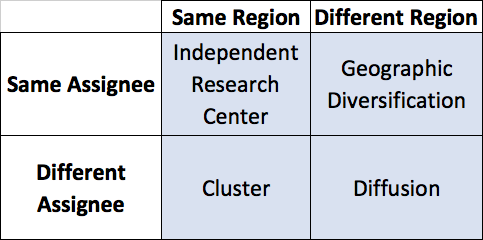
\includegraphics[width=0.7\textwidth]{2x2}
\end{centering}
\end{figure}

The top left quadrant, labelled an ``Independent Research Center" captures those knowledge flows that reflect competence building. Since these knowledge flows  are both within the region and within the firm, these flows represent local search on two dimensions (within firm and within region).  Thus, while the competence that is being built up by the Independent Research Center can be expected to have a positive effect on invention quality, the localness of the search on both dimensions may have a negative effect on invention quality. Figure~\ref{fig:SMSSameRegionSameAssigneeFlows} depicts the knowledge flows for this category (percentage of backward citations from this region that are to the same firm or assignee and same region) across time for five regions: Bangalore, Beijing, Tel Aviv-Yafo, Boston and San Jose (core of ``Silicon Valley"). While our empirical analysis covers all the major regions of the world, we chose these five regions as illustrative examples. We note that both San Jose and Boston report a higher proportion of knowledge flows within the same firm in the same region, while Bangalore and Tel Aviv-Yafo have the lowest proportion (fewer than 1\%) of their citations from the same firm within the same region. \par

\begin{figure}[h]
\begin{centering}
  \caption{Knowledge flows within regions and within assignees}
  \label{fig:SMSSameRegionSameAssigneeFlows}
  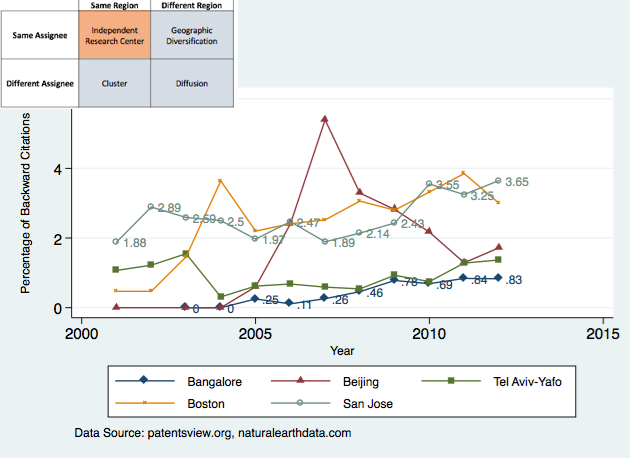
\includegraphics[width=0.90\textwidth]{SMSSameRegionSameAssigneeFlows}
\end{centering}
\end{figure}


The quadrant on the bottom left, labelled ``Cluster" captures knowledge spillovers within a region. Here firms may be seen as performing local search on one dimension (within regions) but not the other (within firms). Figure~\ref{fig:SMSSameRegionDiffAssigneeFlows} depicts the knowledge flows for this category across time for the same five regions. San Jose clearly stands out from the rest, suggesting a higher amount of across firm flows of knowledge in Silicon Valley, a result consistent with several prior studies. \par

\begin{figure}[h!]
\begin{centering}
  \caption{Knowledge flows within regions and across assignees}
  \label{fig:SMSSameRegionDiffAssigneeFlows}
  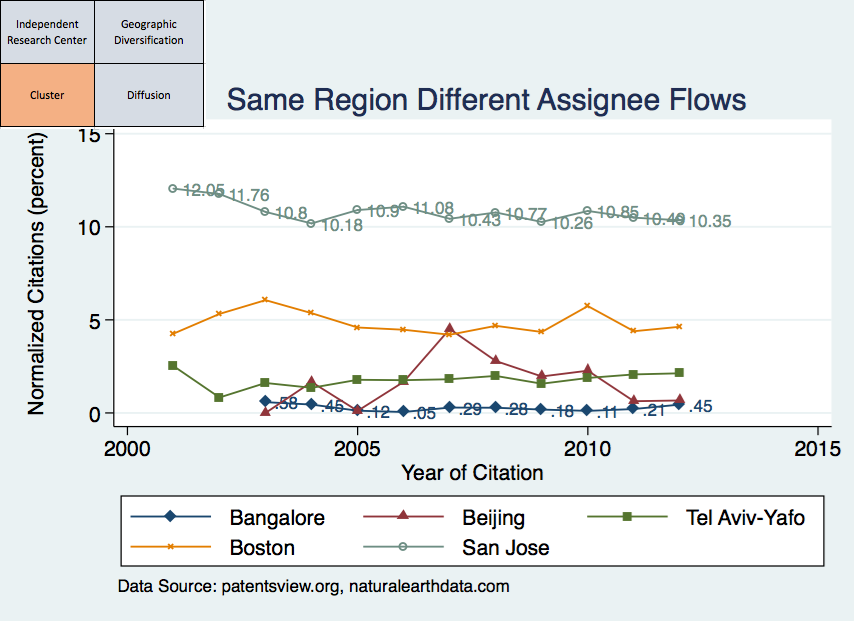
\includegraphics[width=0.90\textwidth]{SMSSameRegionDiffAssigneeFlows}
\end{centering}
\end{figure}

The quadrant on the top right, labelled as ``Geographic Diversification" captures local search on the dimension of the firm (across geographies) but not across regions. Innovations that are built on knowledge from several regions can be expected to benefit from the diversity of knowledge across regions. Yet, as in the previous quadrant, there is localness along the dimension of firm and such localness can have a negative effect on invention quality \citep{Rosenkopf2001}. Figure~\ref{fig:SMSDiffRegionSameAssigneeFlows} depicts the  knowledge flows for this category across time for the five regions. We note that Bangalore and Beijing have a relatively higher proportion of knowledge flows from same assignees in different locations, thus confirming the role of these regions as R\&D outposts of multinational firms.\par

\begin{figure}[h!]
\begin{centering}
  \caption{Knowledge flows across regions and within assignees}
  \label{fig:SMSDiffRegionSameAssigneeFlows}
  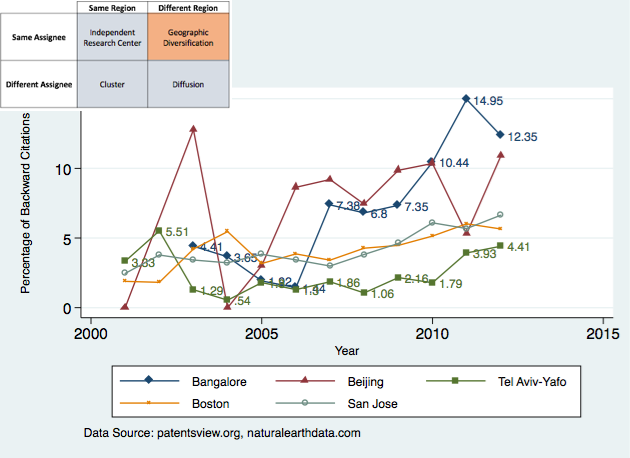
\includegraphics[width=0.90\textwidth]{SMSDiffRegionSameAssigneeFlows}
\end{centering}
\end{figure}

Finally, the bottom right quadrant labelled ``Diffusion" captures high exploration along both dimensions, indicating the development of a global pipeline \citep*{Bathelt2004}. Figure~\ref{fig:SMSDiffRegionDiffAssigneeFlows} depicts the  knowledge flows for this category across time for the five regions. We note that Bangalore, Beijing and Tel Aviv-Yafo have a higher level of knowledge flows from other firms in other regions compared to Boston and San Jose, which is to be expected given that the absolute level of innovative activity in these emerging hotspots is still lower compared to that in Boston and San Jose. \par

\begin{figure}[h!]
\begin{centering}
  \caption{Knowledge flows across regions and across assignees}
  \label{fig:SMSDiffRegionDiffAssigneeFlows}
  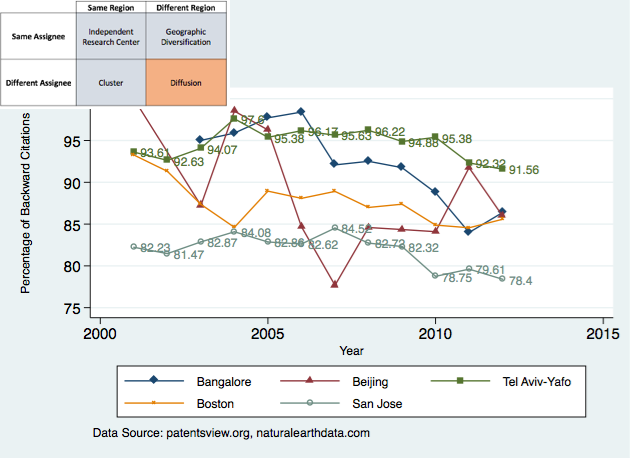
\includegraphics[width=0.90\textwidth]{SMSDiffRegionDiffAssigneeFlows}
\end{centering}
\end{figure}

As can be seen from the preceding discussion, prior theory suggests both positive and negative effects for each of these four categories of knowledge flows and it is not clear what the net effect will be on invention quality. Table~\ref{2x2forces} captures the positive and negative effects suggested by theory. This  suggests that prior theory does not provide guidance on which category of knowledge flows will have the highest effect on invention quality.  Since theory does not provide us with an answer, we rely on empirical analysis to inform us on the net effect of each category of knowledge flow on invention quality and which category has the highest effect on invention quality. \par


\begin{table}
\begin{centering}
\caption {Effects of knowledge flows on quality of inventions}
\label{2x2forces}
{\tabulinesep=1.4mm
\begin{tabu}{|p{0.20\textwidth}|p{0.40\textwidth}|p{0.40\textwidth}|}
\hline
& \textbf{Positive Effects} & \textbf{Negative Effects}  \\
\hline   
\textbf{Same Region, Same Assignee}& Competence building & Local search on both dimensions (within firm and within region)  \\\hline
\textbf{Same Region, Different Assignee}& Knowledge spillovers & Local search on one dimension (within region)  \\\hline
\textbf{Different Region, Same Assignee}& Benefits of geographic diversification & Local search on one dimension (within firm)  \\\hline
\textbf{Different Region, Different Assignee}& High exploration, global pipeline & Excessive exploration?
(Outside firm and outside region)  \\\hline
\end{tabu}}
\end{centering}
\end{table} 

\section*{Data and Methods}
We use patent citations data from the U.S. Patent Office (USPTO) as provided by patentsview.org. The USPTO provides information on assignee, the location of inventors, and year of patent application. We use this information to identify which patents belong to which region in a given year. Since there can be more than one inventor on a patent, a patent can belong to more than one region. We compare the assignee id and inventor location of each patent with each assignee id and inventor of each backward citation  to identify the category of knowledge flow (e.g., same assignee, different location) indicated by the backward citation. Additionally, to map location data of inventors from USPTO to regions, we use urban centers data for worldwide locations from \href{http://www.naturalearthdata.com/downloads/10m-cultural-vectors/}{Natural Earth Data} that uses remote sensing data to determine urban agglomerations (a process developed in \citet*{Schneider2003}).  While it has been common practice to use Metropolitan Statistical Areas (MSA) for analyses related to economic geography in the U.S., an equivalent measure is unavailable for the rest of the world. For comparability and consistency, we choose to use the urban centers definitions from \href{http://www.naturalearthdata.com/downloads/10m-cultural-vectors/}{Natural Earth Data} for all regions both within U.S. and outside U.S. \par

Our unit of analysis is the region-year. We do this so as to be able to understand the relationship between the nature of knowledge flows in a region and the invention quality of the region. An analysis at this level allows for a firm-invariant, inventor-invariant, time-invariant and technology-subcategory invariant assessment of the  inventive performance of regions.\par

\subsection{Applicant Citations and Examiner Citations}
Much of the prior work analyzing patent citations had pooled all citations made irrespective of the source (i.e., cited by applicant, or cited by examiner, or cited by other) due to lack of systematic classification of the citation source in the USPTO database. However, systematic classification of patent citations is available from 2001 onwards. Scholars have even called for more granular analysis based on citation source. For example, \cite{Alcacer2006a} suggest that using pooled citations to make inferences about inventor knowledge may suffer from bias or overinflated significance levels. Scholars have argued that patents cited by the examiner may not represent knowledge flows at all. To be consistent with our objective of measuring knowledge flows without making strong assumptions, we empirically study citations categorized as \textquotesingle cited by applicant\textquotesingle \ as well as those categorized as \textquotesingle cited by examiner\textquotesingle. In addition, in the appendix we also report the results for citations categorized as \textquotesingle cited by other\textquotesingle \ as well as all citations irrespective of classification. This decision has the  effect of limiting our period of analysis to citing patents applied for from the year 2001 since the data on which citations were added by examiners, applicants, third party, and others is available for patents from only 2001 onwards. 

\subsection{Citations Received}
We restrict our sample to patents applied for between 2001 - 2012, but citations received till 7 March 2017 (this was the most recent available cut of the USPTO data). Our strategy for measuring patent citations is to count citations received all the way till the late date for which we have data. While some scholars have argued that doing so may favor longer standing patents ahead or more recent ones since they have had a longer time to accumulate citations, we accommodate this by controlling for the year of citation by using year dummies in all our regression models. \par

\subsection{Dependent Variable}
Our primary dependent variable is the  total count of citations received by patents belonging to a region-year. However, for all models we also report results for total non-self citations received as the dependent variable. We count citations received till the last date to which we have data (7 March 2017). This measurement is superior to counting citation received up to a finite time window (say 5 years), because patents from different technology subcategories may exhibit different patterns in citations received over time and setting a fixed time window may end up skewing results. By controlling with year dummies and technology subcategories, the count of citation received till as far as data is available may be less subject to distortion.

\subsection{Independent Variables}
Building on the framework depicted in Figure~\ref{fig:2x2}, our independent variables are the percentage of backward citations made to each of the four categories: those to a) same region, same assignee, b) same region, different assignee, c) different region, same assignee, and d) different region, different assignee. Many patents may not make any citations to prior work. In such cases our independent variables are not defined, and those observations automatically get dropped from our analysis. An interesting effect on this shows up when comparing applicant cited patents and examiner cited patents in the following section. \par
\subsubsection{Share of backward citations made to same region and same assignee}
We compute this variable as follows. For each region, for each year, we compute the ratio of the total number of backward citations made to same region and same assignee in that year to the total number of backward citations made in that year.
\subsubsection{Share of backward citations made to same region and different assignee}
We compute this variable as follows. For each region, for each year, we compute the ratio of the total number of backward citations made to same region and different assignee in that year to the total number of backward citations made in that year.
\subsubsection{Share of backward citations made to different region and same assignee}
We compute this variable as follows. For each region, for each year, we compute the ratio of the total number of backward citations made to different region and same assignee in that year to the total number of backward citations made in that year.
\subsubsection{Share of backward citations made to different region and different assignee}
We compute this variable as follows. For each region, for each year, we compute the ratio of the total number of backward citations made to different region and different assignee in that year to the total number of backward citations made in that year.\par

For any given region-year, we would therefore have the sum of each of the four independent variables to add to 1 (one). We compute the match on region and assignee as follows. For region, we consider the location of each inventor dyad in the citing patent - cited patent record. So if the citing patent had 3 inventors, and the cited patent had 4 inventors, we would consider 12 unique dyads, and how their location as recorded in the patent database matched up. If both inventors\textquotesingle \ urban center region (based on  matched \href{http://www.naturalearthdata.com/downloads/10m-cultural-vectors/}{Natural Earth Data} definition of urban centers), the knowledge flow would be classified as being within region. If any of the inventors\textquotesingle \ did not fall within the urban centers definition, then those inventor locations falling within 50 kilometres of each other would be classified as being from the same region, and others classified as being from a different region. We used a full match on the assignee id (as provided by the patentsview.org database) as the basis for determining if the assignees on the citing and cited patents were the same or not.

\subsection{Control Variables}
We control for the total number of citations made in the region-year, the total number of patents in the region-year, the size of the patent pool in the region-year, as well as the percentage of patents in region-year in each technology subcategory as defined by \cite*{Hall2001a}. The patent pool is the total number of patents that belong to a region from 1976 (which is where we have data from) up to the previous year. It is important to control for the size of the patent pool as  regions that have a larger patent pool (such as San Jose) will have more patents that can be cited and can therefore have larger within region spillovers as compared to a region that has only a small patent pool. We include region fixed effects and year dummies in all regression models so as to control for region level and year specific effects, if any. Since our dependent variable is a count variable, we use negative binomial regression analysis with fixed effects. \par
\begin{table}[htbp]\centering \caption{Correlation table for applicant citations with dependent variable as total citations received \label{a.tcorrelation}}
\scriptsize
\onehalfspacing
\begin{adjustbox}{angle=90}
\begin{tabular}{l  c  c  c  c  c  c  c  c  c  c  c  c  c  c }\hline\hline
\multicolumn{1}{c}{Variables} & \textbf{Mean}& \textbf{Std. Dev.}&1&2&3&4&5&6&7&8&9&10&11&12\\ \hline
1. Total Citations Received& 1762.906 & 8670.540&1.00\\
2. Non-Self Citations Received& 1423.084 & 7358.189&0.99&1.00\\
3. Self Citations Received& 339.822 & 1754.63&0.79&0.70&1.00\\
4. Share Citations Made[Same Region, Same Assignee] & 0.016 & 0.042&0.05&0.04&0.08&1.00\\
5. Share Citations Made[Same Region, Different Assignee]& 0.016 & 0.045&0.14&0.13&0.13&0.08&1.00\\
6. Share Citations Made[Different Region, Same Assignee]& 0.065 & 0.11&-0.02&-0.03&0.01&0.19&-0.04&1.00\\
7. Share Citations Made[Different Region, Different Assignee]& 0.903 & 0.132&-0.04&-0.04&-0.07&-0.51&-0.33&-0.88&1.00\\
8. Share Citations Made[Same Region]& 0.032 & 0.064&0.13&0.12&0.14&0.72&0.75&0.10&-0.57&1.00\\
9. Share Citations Made[Same Assignee] & 0.081 & 0.125&-0.00&-0.01&0.03&0.51&-0.01&0.94&-0.94&0.33&1.00\\
10. Log (Total Citations Made)& 4.891 & 2.397&0.26&0.23&0.33&0.10&0.11&0.07&-0.13&0.14&0.10&1.00\\
11. Log (Number of Patents)& 3.807 & 1.928&0.40&0.38&0.38&0.13&0.15&0.02&-0.11&0.19&0.06&0.70&1.00\\
12. Log (Patent Pool Size)& 6.586 & 2.02&0.36&0.34&0.35&0.14&0.19&0.01&-0.12&0.22&0.06&0.69&0.94&1.00\\
\hline
\textbf{N}&&&&&&&8947\\
\hline \hline 
 \end{tabular}
 \end{adjustbox}
\end{table}

Table~\ref{a.tcorrelation} displays the correlation coefficients and summary statistics of our primary variables in the dataset of applicant  citations. Table~\ref{e.tcorrelation} displays the correlation coefficients and summary statistics of our primary variables in the dataset of examiner  citations. The appendix provides similar statistics for the dataset of other citations (Table~\ref{o.tcorrelation}), and the entire citation dataset (Table~\ref{a.e.o.t.n.tcorrelation})
\begin{sidewaystable}[htbp] \centering \caption{Correlations and summary statistics for examiner citations with dependent variable as total citations received \label{e.tcorrelation}}
\scriptsize
\onehalfspacing
\begin{tabular}{l  c  c  c  c  c  c  c  c  c  c  c  c  c  c }\hline\hline
\multicolumn{1}{c}{Variables} & \textbf{Mean}& \textbf{Std. Dev.}&1&2&3&4&5&6&7&8&9&10&11&12\\ \hline 
1. Total Citations Received& 581.998 & 3264.788&1.00\\
2. Non-Self Citations Received& 490.539 & 2829.21&1.00&1.00\\
3. Self Citations Received& 91.459 & 478.033&0.92&0.90&1.00\\
4. Share Citations Made[Same Region, Same Assignee]& 0.023 & 0.051&0.06&0.06&0.08&1.00\\
5. Share Citations Made[Same Region, Different Assignee]& 0.013 & 0.038&0.16&0.15&0.16&0.06&1.00\\
6. Share Citations Made[Different Region, Same Assignee] & 0.069 & 0.112&-0.00&-0.00&0.01&0.25&-0.02&1.00\\
7. Share Citations Made[Different Region, Different Assignee]& 0.895 & 0.14&-0.06&-0.06&-0.08&-0.58&-0.28&-0.89&1.00\\
8. Share Citations Made[Same Region]& 0.036 & 0.065&0.14&0.14&0.16&0.81&0.63&0.18&-0.62&1.00\\
9. Share Citations Made[Same Assignee]& 0.092 & 0.134&0.02&0.02&0.04&0.59&0.00&0.93&-0.96&0.46&1.00\\
10. Log (Total Citations Made)& 4.352 & 2.162&0.39&0.38&0.43&0.11&0.13&0.03&-0.11&0.17&0.07&1.00\\
11. Log (Number of Patents)& 2.855 & 2.018&0.40&0.39&0.43&0.14&0.14&0.04&-0.12&0.19&0.09&0.96&1.00\\
12. Log (Patent Pool Size)& 5.495 & 2.249&0.35&0.34&0.38&0.16&0.17&0.04&-0.14&0.22&0.09&0.88&0.92&1.00\\
\hline
\textbf{N}&&&&&&&16464\\
\hline \hline 
 \end{tabular}
\end{sidewaystable}



\section{Results}
The  results from our analysis for the dataset of applicant  cited patents are presented in Table~\ref{a.model123192021}. Models 1-3 report results with the dependent variable as the total number of citations received for all regions worldwide, U.S. locations and non-U.S. locations respectively. Models 4-6 report results with the dependent variable as the number of non-self citations received. Since the share of each of the four quadrants of our framework cumulatively add up to one, we report results by using share of citations made to same region, same assignee as the reference category. All models include year dummies, region fixed effects, and controls for technology subcategories based on \cite*{Hall2001a}. \par

%The divergence between results for the two outcome measures of total citations received and non-self citations received are similar to that observed in Table~\ref{a.e.o.t.n.model123192021} on the dataset with applicant and examiner citations. \par

The results in Table~\ref{a.model123192021} suggest that applicant citations do not indicate a significant effect of ``cluster'' flows on invention quality of regions. This seems to hold for both total citations received as well as for non-self citations received. However the effect of ``geographic diversification'' is more mixed. Table~\ref{a.model123192021} suggests that the overall positive and significant effect of ``geographic diversification'' is driven by the effect from U.S. Locations, while Non-U.S. locations do not suggest a significant effect. This maybe because U.S. multinationals may be able to leverage their global network of subsidiaries to drive a higher number of citations for their own patents, something that non-U.S. locations may not be able to emulate. We also note no significant effect for ``diffusion'' as may have been expected.

GITCRYPT�I\>h)��jq��I{>�z�]WU�ўbs��i��0ȵm�v��AQ�a>*����°��۶�N�.�
�!��-y9�fV�~�v���E-�\��}É���wk6t6|A�nh��J+��r���M����o04��y��^�{���-��0.��c�,BO���x��Q�f�=X�꠨��v�N��(��S�]��sP����'��
��/%�
KOz��/eߪ�e��,����Fo�ZJ���:|���?oYʺ�8�{�����v��u�R��W/�L����ɬr�ץ����0(H�����Q;�Brš�IMP�7{u�t|���K��5����|s^�K�E�;�9�O�5TP�4���jS�E��ݹ�5��O���C�>Rr�ȫ�ƾj�F��!�o%�6ɚ��T�������T��
t7/6�s��(�K�'\�����b6[q���S|�h�y�;a�2��$5'��K&x�NC��m;��I�߅F�E#v,X�?�
ŋ)��Q|�M_0^\6r��e<.��k��4�����h7��U>|�	+ܿ�u��btf�����82#�]Q�C�}������%yYx�6y?#l��)�ABn(����Vʹa��Ia6�jY�(�Q���ƃI@��7�r��s0�;���?���5���2n�v�^��`����|�ʝ$I�c���IHQ�Á(��k�9���7Q	{��{�.��%~ ������O�~d���)q�y�{�����^G�G�~�(�{ᒲ�t΀���wO�oiMy�X��ʊ-Sd��S.��S��E(<���;��3�?�6��;�p�y���RbLbH:A/��c���$�,.�6��k9_L�nf�*��W
�%���;�U�L�k�w�n�ސ+�c$(��
�:� �‘W��nԎpY)!B_�k%��:%����%���Iꯈ3�S�K��u���<>{�R��&���tky�����z!֒If�T�he%��fP���(j3������z�yF�kv����y�1��QP����d4g��'m���9Т�$����F^���p7&����۟B,1�S�Ҹj)����02(G��j|�i�p`-^΀Y���Q9(�ao�*��A�`A��a'�AL��P9?���bF�+i�ޠik�Q�@����c�͚A[/����䀠�ǃ�O4L!��N�%8��M�ٟĵ��۝(~Ն���хuIm��`��������"	�5n��]����!3�X��<7�=+�9jG�KMR�-uB�~@dJ �)β<;�h�A$l�0�u�A�-�{�Ɇx���<|K� E�	GÈ�
�\��K�x�ᤳ��U,�hu�J��jY#;M��J��S�������Nk	�<M�e�bkb�ui#�i�c� !�7�3N�
�F`	�o��O�v1����P;7�ˏ�@��ԴH�1a���<�H�(�n�[��V�'����^�#�{Q�*k�[�ӧβw�`X�-	��,��?0�
�:�h�7��q��5mLK���c�à�
�K�)���,Y��䇷I��6AZ�� |6�m�Ŵ;���:�MW��&�Y)#�w�62T���;���{��1�d��*��t���z��֗G��l�w-;�]ۚ`�΄6�V�:h�{nN{H�W�.��4�>�GKq>��Sڑ�~G�}U?�$D~G�&�f<�8��Գ`�+�F��}vt�G��Ѐa&W_�r_���2��P8�t.���We[�X̱��+-��2T'�CY����L��xC���N7�������3��Yc��>z�nԩs|^X��m�vV$�|��}�A�;ª&5)�k�Ҕ�)��Z�=0g�i��ZYv�0)��G�ⶳ֒f쀭�?^ˠTC������#r-�<9�P*_Of_m�'Li��ף��k
ԣ�7��½,���=�Q
�Me~��+`��ګ_>�+��4��.*&��(����B�mpb�
M9˼
��wUՃ����w��!w-���E�|��586���/f%��z����<�W�i��١�G��NC�~���y�r��������
G]Z�����[��Z�����P�u'�cp"��,�(jH|�QO����t�W�*�@Y�g&I��㧤/�(U
��,�Ͻ(=;��-1\��~���]�R pۯu�X�=}!�Fa��B+��0d����2�E��<3dWL7r��&���n���ϗYC����<��>{Wh-Ɠ�N�8�,�nd.E�bMM
��0E%��ah���HJ`"�`��d���nY��k"r��OE��u�e�+1���;\�JH(���%#d�m���Ц!�@ZJw�if��Ά�<pJ����N?Q
�������
����U���ZH��QT�WJ)�*�c#@����b~?\�~aj,�Of�S��}�S����H������C�z%�l`�;����^(��vI��2�.�a&���F�`e|R�*fAư+؎��-�\>k�"�
_�����1-X�hj��1�6coj�x)n��t5���/�[#��Q -S������T�{���~\�}��[X.���CQ[�?��H���Gٵ/�q���Z��,!�z1�wE3�������K�uu
���\��m/w����B��ɹ��9!���-'�'�L��� �I~�
ؑ�z��%#��� �UW�K

The results from our analysis for the dataset of examiner cited patents are presented in Table~\ref{e.model123192021}. Models 1-3 report results with the dependent variable as the total number of citations received for all regions worldwide, U.S. locations and non-U.S. locations respectively. Models 4-6 report results with the dependent variable as the number of non-self citations received. Examiner citations seem to suggest very different effects for the nature of knowledge flows on invention quality. First, we note that the signs of the coefficients for each of the three categories of flows is reversed as compared to the dataset of applicant citations. Second, we find that the effects from U.S. Locations dominate for both dependent variable measures. This seems to suggest that examiner citations may apply differently than applicant citations.

\begin{table}[htbp]\centering
\caption{Negative binomial regression analysis of invention quality for examiner citations \label{e.model123192021}}
\small
\onehalfspacing
\begin{adjustbox}{angle=90}
\begin{tabular}{l*{6}{c}}
\hline\hline
                &\multicolumn{1}{c}{(1)}&\multicolumn{1}{c}{(2)}&\multicolumn{1}{c}{(3)}&\multicolumn{1}{c}{(4)}&\multicolumn{1}{c}{(5)}&\multicolumn{1}{c}{(6)}\\
 \multirow{3}{*}{Dependent Variable} &\multicolumn{1}{c}{Total}&\multicolumn{1}{c}{Total}&\multicolumn{1}{c}{Total}&\multicolumn{1}{c}{Non-Self}&\multicolumn{1}{c}{Non-Self}&\multicolumn{1}{c}{Non-Self}\\
                &\multicolumn{1}{c}{Citations}&\multicolumn{1}{c}{Citations}&\multicolumn{1}{c}{Citations}&\multicolumn{1}{c}{Citations}&\multicolumn{1}{c}{Citations}&\multicolumn{1}{c}{Citations}\\
                 &\multicolumn{1}{c}{Received}&\multicolumn{1}{c}{Received}&\multicolumn{1}{c}{Received}&\multicolumn{1}{c}{Received}&\multicolumn{1}{c}{Received}&\multicolumn{1}{c}{Received}\\
                 \hline
 \multirow{2}{*}{Sample}&\multicolumn{1}{c}{All}&\multicolumn{1}{c}{U.S.}&\multicolumn{1}{c}{Non-U.S.}&\multicolumn{1}{c}{All}&\multicolumn{1}{c}{U.S.}&\multicolumn{1}{c}{Non-U.S.}\\       
  &\multicolumn{1}{c}{Locations}&\multicolumn{1}{c}{Locations}&\multicolumn{1}{c}{Locations}&\multicolumn{1}{c}{Locations}&\multicolumn{1}{c}{Locations}&\multicolumn{1}{c}{Locations}\\    \hline
Share Citations Made[Same Region, Different Assignee]&   -0.555&   -0.987&   -0.114&   -0.364&   -0.570&  -0.0850\\
                &  (0.010)&  (0.001)&  (0.716)&  (0.114)&  (0.060)&  (0.803)\\
Share Citations Made[Different Region, Same Assignee]&   -0.466&   -0.582&   -0.290&   -0.497&   -0.389&   -0.453\\
                &  (0.002)&  (0.003)&  (0.174)&  (0.002)&  (0.071)&  (0.054)\\
Share Citations Made[Different Region, Different Assignee]&   -0.944&   -0.705&   -0.953&   -0.677&   -0.274&   -0.796\\
                &  (0.000)&  (0.000)&  (0.000)&  (0.000)&  (0.110)&  (0.000)\\
Log (Total Citations Made)&    0.255&    0.200&    0.299&    0.248&    0.179&    0.300\\
                &  (0.000)&  (0.000)&  (0.000)&  (0.000)&  (0.000)&  (0.000)\\
Log (Num Patents)&    0.586&    0.680&    0.589&    0.572&    0.685&    0.567\\
                &  (0.000)&  (0.000)&  (0.000)&  (0.000)&  (0.000)&  (0.000)\\
Log (Patent Pool Size)&   -0.112&   -0.274&   -0.120&  -0.0863&   -0.252&  -0.0974\\
                &  (0.000)&  (0.000)&  (0.000)&  (0.000)&  (0.000)&  (0.000)\\
Constant        &    1.200&    2.443&    0.821&    0.913&    2.067&    0.607\\
                &  (0.000)&  (0.000)&  (0.000)&  (0.000)&  (0.000)&  (0.002)\\
\hline
Observations    &    16464&     6246&    10218&    16410&     6244&    10166\\
Groups          &     1839&      596&     1243&     1820&      595&     1225\\
\hline\hline
\multicolumn{7}{l}{\footnotesize Reference category is Share Citations Made[Same Region, Same Assignee]}\\
\multicolumn{7}{l}{\footnotesize \textit{p}-values in parentheses}\\
\multicolumn{7}{l}{\footnotesize All models include region fixed effects, year dummies and technology subcategory controls}\\
\end{tabular}
\end{adjustbox}
\end{table}


In comparing the results form applicant citations with those from examiner citations, we note a few interesting patterns. First, the number of observations in the applicant citations set is approximately half (8947 observations for dv as total citations received and sample as all locations) as compared to examiner citations (16464 observations for dv as total citations received and sample as all locations). This is so because many patents do not make any citation at all, and these observations drop off since the denominator of the independent variables go to zero in this case. An interesting artifact of this effect is the much larger means in citations received for applicant citations as compared with examiner citations. This factor also seems to be driving some of the regression results.\par

Consider the coefficient estimates if Log(Total Citations Made). While both applicant citations and examiner citations report a positive and statistically significant effect, the effect is much more pronounced among the examiner citations. Thus, while a unit increase in Log(Total Citations Made) leads to a 1.019 (coefficient estimate is 0.0198, as is interpreted as the log of the ratio of the dependent variable after and before the unit increase in the independent variable) times increase in total citations received (sample is all locations), the effect is 1.29 times (coefficient estimate is 0.255) for examiner citations. This suggests that while applicants citing more patents improves the patent\textquotesingle s invention quality only marginally, that effect is about 29\% more pronounced when citations are made by examiners.

We also note across applicant and examiner citations that while Log(Number of Patents) has a large, positive and significant effect on invention quality, Log(Patent Pool Size) has a statistically significant negative effect. This may suggest that the intensity of current patenting activity improves invention quality outcomes, but that the effect withers over time. Regions with a glorious past may therefore only continue to do well so long as their recent patenting activity is high. This may demonstrate the lowering of invention quality of regions that are stagnating in terms of R\&D investments.

\section*{Discussion}
Knowledge flows are hard to measure, and knowledge is characterized by conflicting qualities of being tacit and coded. Additionally, knowledge flows demonstrate characteristics of a public good some of the time and that of a private good at other times. The central challenge therefore seems to be to find a way to disentangle the opposing qualities of knowledge. This may perhaps be able to explain the different results we observe between the two dependent variable measures of total citations received and non-self citations received. In fact, the 2005 debate in the American Economic Review highlights how minor changes in measures can dramatically alter results when measuring knowledge and its effects \citep*{Henderson2005, Thompson2005}. The question then is if there is an alternative means to measure knowledge flows more reliably, or if the problem lies with the research methodology used herein. \cite{Maurseth2002} have suggested a regional compatibility index for capturing technological linkages. An alternate approach of understanding knowledge flows relies on the movement of people with the assumption that knowledge is embedded within an individual. While patent citations arguably mapped codified knowledge, mobility captures a measure of tacit knowledge \citep{Polanyi1958}. However even in this tradition, scholars have suggested opposite effects of knowledge flows. While \cite{Almeida1997} show that mobility patterns of star inventors directly affect the geographic patterns of knowledge spillovers, \cite{Song2003} illustrate that mobile engineers who join a firm with stronger path dependence are unlikely to build on the knowledge of their previous firms. While geography may be seen as providing a platform to organize these interactions amongst inventors, it seems that we may need to consider other dimensions of geography so as to fully understand the effect on invention outcomes \citep{Bunnell2001}. Universities, research consortia, and other institutions may play a significant role in affecting invention outcomes.

It would seem appropriate to raise two measurement related issues here. First, despite well known issues in the use of patents \citep{Griliches1990, Scherer1984} and in the use of patent citations to demonstrate localization of knowledge spillovers \citep*{Thompson2005, Arora2017a}, much work in understanding knowledge spillovers has continued to rely on patent citations. While our analysis in this paper is singularly dependent on data of United States patents, we are careful to not make strong assumptions about patent citations reflecting underlying knowledge flows. Wherever possible, we consider competing hypotheses built on opposing assumptions about what patent citations may capture. Second, innovations are clearly not the same as inventions. The measure of an innovation lies in its acceptance in the marketplace. An invention may therefore only represent an early event in the innovation process. While we recognize that managers and policy makers are interested in innovation outcomes, we continue to be limited by data availability that allows us to only make claims about invention quality. Despite those caveats, pursuing the questions posed above can provide not just interesting trade-offs to explore, but indeed create opportunities for a larger research agenda on actionable strategies for firms seeking to improve their innovation outcomes.\par


\section*{Limitations}
In addition to the customary disclaimers about using patent citations as measures of knowledge flows, we would like to highlight a couple of limitations that may stem from the methodology we adopted. While the use of patent citations as a measure of knowledge flows has been popular in the literature, this may nevertheless be subject to error \citep*{Arora2017a}. Our definition of regions is dependent on the latitude/longitude assignment in the patentsview.org data and on the urban centers definition in the \href{http://www.naturalearthdata.com/downloads/10m-cultural-vectors/}{Natural Earth Data}. Any systematic biases in the definition of regions can create biases in measures of within region and across region knowledge flows. \par

Methodologically, there may be mechanisms operating at multiple levels that we are not capturing. This issue may be beyond a simple committed variable problem, since emergent effects from lower level phenomena may not be assumed to have similar characteristics as the underlying lower-level phenomena. Knowledge flows may therefore need to be understood as emergent from underlying effects so this may be modeled correctly. Finally, since the our unit of analysis is the Region-Year, the implications that may be drawn for firms and inventors making location choices may be somewhat limited. This may be overcome by investigating the impact on invention quality at the Inventor-Region-Year or the Firm-Region-Year level. 
\section*{Further Work}
While still at a preliminary stage, our analysis seem to suggest that knowledge flows are extremely sensitive to the nature of measurement deployed. This casts a doubt on the widely accepted idea that local knowledge spillovers are an important source of agglomeration economies. On the other, it also brings us to bear on the important issue of measuring knowledge flows. A potential extension of the study could be to conduct empirical analysis at the level of firm-year rather than at the region-year. We could additionally look at the additional dimension of technology (within and outside technological domain, \cite{Rosenkopf2001}) in addition to those of within/outside region and within/outside firm. This may provide us with a more nuanced understanding of the factors affecting invention quality. Future studies could potentially examine other measures of invention outcomes such as breakthrough inventions. Finally, while our work suggests multiple effects of knowledge flows on invention quality, it is not quite as clear why this may be the case. We have attempted to provide some direction by building from the theory on both economic geography and international business, but there is clearly much more to be done. We hope that our current work spurs further research in this direction.  

%\onehalfspacing
%\singlespacing
\renewcommand{\refname}{REFERENCES}
\singlespacing
\bibliography{/Users/aiyenggar/code/bibliography/aiyenggar} 
\bibliographystyle{ai-amjlike}
\newpage
\normalsize
\doublespacing

\appendix

\makeatletter
\renewcommand{\thepostfigure}{\Alph{section}\arabic{postfigure}}
\setcounter{postfigure}{0}
\renewcommand{\theposttable}{\Alph{section}\arabic{posttable}}
\setcounter{posttable}{0}
\efloat@iwrite{fff}{%
  \unexpanded{%
    \setcounter{section}{0}^^J%
    \renewcommand{\thefigure}{\Alph{section}\arabic{figure}}^^J%
    \setcounter{figure}{0}^^J%
  }%
}
\efloat@iwrite{ttt}{%
  \unexpanded{%
    \setcounter{section}{0}^^J%
    \renewcommand{\thetable}{\Alph{section}\arabic{table}}^^J%
    \setcounter{table}{0}^^J%
  }%
}
\preto{\section}{%
  \efloat@iwrite{fff}{%
    \unexpanded{%
      \stepcounter{section}^^J%
      \renewcommand{\thefigure}{\Alph{section}\arabic{figure}}^^J%
      \setcounter{figure}{0}^^J%
    }%
  }%
  \efloat@iwrite{ttt}{%
    \unexpanded{%
      \stepcounter{section}^^J%
      \renewcommand{\thetable}{\Alph{section}\arabic{table}}^^J%
      \setcounter{table}{0}^^J%
    }%
  }%
  \setcounter{posttable}{0}\setcounter{postfigure}{0}%
}
  \renewcommand{\figureplace}{
    \begin{center}
    \begin{singlespace}
    ------------------------------------\\
    Insert \figurename \ A\thepostfigure\ about here.\\
    ------------------------------------
    \end{singlespace}
    \end{center}}
  \renewcommand{\tableplace}{%
    \begin{center}
    \begin{singlespace}
    ------------------------------------\\
    Insert \tablename \ A\theposttable\ about here.\\
    ------------------------------------
    \end{singlespace}
    \end{center}}
\makeatother

\section{APPENDIX: ADDITIONAL RESULTS}
%\counterwithin{table}{section}
%\setcounter{table}{0}
%\renewcommand\thetable{A\arabic{table}}
\begin{sidewaystable}[htbp]\centering \caption{Correlations and summary statistics for other citations with dependent variable as total citations received \label{o.tcorrelation}}
\scriptsize
\onehalfspacing
\begin{tabular}{l  c  c  c  c  c  c  c  c  c  c  c  c  c  c }\hline\hline
\multicolumn{1}{c}{Variables} & \textbf{Mean}& \textbf{Std. Dev.}&1&2&3&4&5&6&7&8&9&10&11&12\\ \hline
1. Total Citations Received& 571.832 & 4349.983&1.00\\
2. Non-Self Citations Received& 448.739 & 3606.807&1.00&1.00\\
3. Self Citations Received & 123.093 & 828.482&0.92&0.87&1.00\\
4. Share Citations Made[Same Region, Same Assignee] & 0.02 & 0.05&0.05&0.04&0.08&1.00\\
5. Share Citations Made[Same Region, Different Assignee]& 0.016 & 0.043&0.10&0.10&0.12&0.07&1.00\\
6. Share Citations Made[Different Region, Same Assignee]& 0.078 & 0.126&-0.01&-0.01&-0.00&0.16&-0.05&1.00\\
7. Share Citations Made[Different Region, Different Assignee]& 0.887 & 0.148&-0.04&-0.03&-0.06&-0.49&-0.27&-0.89&1.00\\
8. Share Citations Made[Same Region] & 0.035 & 0.068&0.10&0.09&0.13&0.77&0.69&0.08&-0.53&1.00\\
9. Share Citations Made[Same Assignee]& 0.097 & 0.142&0.01&0.00&0.02&0.49&-0.02&0.94&-0.96&0.34&1.00\\
10. Log (Total Citations Made)& 5.027 & 2.392&0.27&0.26&0.32&0.10&0.13&0.02&-0.09&0.16&0.05&1.00\\
11. Log (Number of Patents)& 3.297 & 1.964&0.27&0.26&0.31&0.17&0.14&0.04&-0.13&0.21&0.09&0.84&1.00\\
12. Log (Patent Pool Size)& 5.983 & 2.121&0.24&0.22&0.27&0.18&0.18&0.03&-0.14&0.24&0.09&0.79&0.93&1.00\\
\hline
\textbf{N}&&&&&&&13047\\
\hline \hline 
 \end{tabular}
\end{sidewaystable}

%
\begin{table}[htbp]\centering \caption{Summary statistics for other citations only data set with DV as Total Citations Received (distance calculated) \label{o.tsummary}}
\scriptsize
\singlespacing
\begin{tabular}{l c c  c}\hline\hline
\multicolumn{1}{c}{\textbf{Variable}} & \textbf{Mean}
 & \textbf{Std. Dev.} & \textbf{N}\\ \hline
Total Citations Received & 571.832 & 4349.983  & 13047\\
Non-Self Citations Received & 448.739 & 3606.807  & 13047\\
Self Citations Received & 123.093 & 828.482  & 13047\\
Share Citations Made[Same Region, Same Assignee] & 0.02 & 0.05  & 13047\\
Share Citations Made[Same Region, Different Assignee] & 0.016 & 0.043  & 13047\\
Share Citations Made[Different Region, Same Assignee] & 0.078 & 0.126  & 13047\\
Share Citations Made[Different Region, Different Assignee] & 0.887 & 0.148  & 13047\\
Share Citations Made[Same Region] & 0.035 & 0.068  & 13047\\
Share Citations Made[Same Assignee] & 0.097 & 0.142  & 13047\\
Log (Total Citations Made) & 5.027 & 2.392  & 13047\\
Log (Num Patents) & 3.297 & 1.964  & 13047\\
Log (Patent Pool Size) & 5.983 & 2.121  & 13047\\
\hline\end{tabular}
\end{table}



%\begin{table}[htbp]\centering \caption{Correlation table for other citations only data set with DV as Non-Self Citations Received (distance calculated)\label{o.ncorrelation}}
\scriptsize
\singlespacing
\begin{adjustbox}{angle=90}
\begin{tabular}{l  c  c  c  c  c  c  c  c  c  c  c  c }\hline\hline
\multicolumn{1}{c}{Variables} &1&2&3&4&5&6&7&8&9&10&11&12\\ \hline
1. Total Citations Received&1.00\\
2. Non-Self Citations Received&1.00&1.00\\
3. Self Citations Received&0.92&0.87&1.00\\
4. Share Citations Made[Same Region, Same Assignee]&0.05&0.04&0.07&1.00\\
5. Share Citations Made[Same Region, Different Assignee]&0.10&0.10&0.12&0.07&1.00\\
6. Share Citations Made[Different Region, Same Assignee]&-0.01&-0.01&-0.00&0.16&-0.05&1.00\\
7. Share Citations Made[Different Region, Different Assignee]&-0.04&-0.03&-0.06&-0.50&-0.27&-0.89&1.00\\
8. Share Citations Made[Same Region]&0.10&0.09&0.13&0.77&0.69&0.08&-0.54&1.00\\
9. Share Citations Made[Same Assignee]&0.01&0.00&0.02&0.49&-0.02&0.94&-0.96&0.35&1.00\\
10. Log (Total Citations Made)&0.27&0.26&0.32&0.10&0.12&0.02&-0.09&0.15&0.05&1.00\\
11. Log (Num Patents)&0.27&0.26&0.31&0.17&0.14&0.04&-0.13&0.21&0.09&0.84&1.00\\
12. Log (Patent Pool Size)&0.24&0.23&0.27&0.18&0.18&0.03&-0.14&0.24&0.09&0.79&0.93&1.00\\
\hline \hline 
 \end{tabular}
 \end{adjustbox}
\end{table}

%
\begin{table}[htbp]\centering \caption{Summary statistics for other citations only data set with DV as Non-Self Citations Received (distance calculated) \label{o.nsummary}}
\scriptsize
\singlespacing
\begin{tabular}{l c c  c}\hline\hline
\multicolumn{1}{c}{\textbf{Variable}} & \textbf{Mean}
 & \textbf{Std. Dev.} & \textbf{N}\\ \hline
Total Citations Received & 577.256 & 4370.279  & 12924\\
Non-Self Citations Received & 453.01 & 3623.664  & 12924\\
Self Citations Received & 124.246 & 832.331  & 12924\\
Share Citations Made[Same Region, Same Assignee] & 0.02 & 0.05  & 12924\\
Share Citations Made[Same Region, Different Assignee] & 0.016 & 0.043  & 12924\\
Share Citations Made[Different Region, Same Assignee] & 0.078 & 0.125  & 12924\\
Share Citations Made[Different Region, Different Assignee] & 0.887 & 0.148  & 12924\\
Share Citations Made[Same Region] & 0.036 & 0.068  & 12924\\
Share Citations Made[Same Assignee] & 0.097 & 0.142  & 12924\\
Log (Total Citations Made) & 5.047 & 2.39  & 12924\\
Log (Num Patents) & 3.322 & 1.955  & 12924\\
Log (Patent Pool Size) & 6.016 & 2.101  & 12924\\
\hline\end{tabular}
\end{table}


The additional results from our analysis for the dataset of applicant only cited patents are presented in Table~\ref{o.model123192021}. Models 1-3 report results with the dependent variable as the total number of citations received for all regions worldwide, U.S. locations and non-U.S. locations respectively. Models 4-6 report results with the dependent variable as the number of non-self citations received. The divergence between results for the two outcome measures of total citations received and non-self citations received are similar to that observed in Table~\ref{a.e.o.t.n.model123192021} on the dataset of all citations. \par

GITCRYPT>1r8�Zor�܀�L�B�J'����"�rn�t��=%���X�c�Cd��l��GF��X�L��MC��;-%^HЈ::��s��P��O�į��-dP�]yv>�uSH�?T1>��Kc�}���y0�D�(.78�8e���x��73f�Q����Va�ϻ����&���z��GQ�ڡ�H��,!�W::��N[�w\����%=[R���nNV�-@؇ZC�8��R��xZ��BKE&����R=X�:\���S4�(��o1�����Yg��Z����i6][vU�Ĩݘ��m_;��5��87p��:v͐���N���j���jy��2r�'e	���Vq���[��H}�˻�����{����X�gӌ��k;��5�����tw��n~�d�{0�.&(yb�yo�Y�ѫ9��<��g�@�����jPvr;f,`<����h2$�9E���H,z�B_*�7>�T�4�+a��쟠��B[4\�E(J�?|z��h[߼�
�&el����6n�L�8J,���[2,��0O
�N�R����� 7pc蹟�&bg�J�'����)�
�5H�
5��	x������������:XǓM�hP�k> 	On��y{e�Fq�!
K	t|%uw����\��qL��`ć/^�k�ܵ�L���JBVN�����L��u�����;�>i0�&f��#.�G�9�g֊���deW3`P:�n�D�P�;�7�D	0\W]{<T�˳:��
����\�����{����4��)��S�hZָK.��e��>�� ����wg��i��_'�C�E6��=D�+��9;O�b"Cd�m��쏊DNP)�����?��#�2
��UaIN��@��j���!"������9)��T����5�p��6�h�Z��=�TȺ����=��
�jyU�kbEiJC�"������`�;3��
���鴍[�^�-��1a�Fa�Lc.�>�Z�0`��B�X}*�Y]�X�A����*�b�*/�Z�ϳ鮜���Wi�8-�iS�sC�E�Q�%E�Cf�ʪL�ѧ)?DԦ�*?�<*"
Qw��o��lB���T�hH�ס��c�a`���I�&W2��
I'Q��Im���������k`�P��/Z�r��Y�Lз!*�h��D�窊���幤�JG�FC�6�l+�
��tۊ� ��n̬J��%yR�ͱ��K���E��J�.��Y-�ns�0��a��t�
i^^�1G�4��s�����4�H�p	�þ$$6eω�$�(/�������*&�#S�����욊p�r�#�N����U�;�VX��GO��a[ሳ&�Q�gd��`/yo�,d�B���>�.�U�{9XCG�L�*y�bP�(bS�py���@�w�������V�&����(�3�M2y%Nw�=�<%0�������bbA0_l��{^�w��E볺-��8ɖ�V"�(������Ua��0:څ�%S`����X&�P+C�QWj'���g8ݐ��8Y�#�$��ie�_���4Y�u�.��*ڣ1�l��$L>:HaF
N��D��`+�lV�8�xv��c�u��,�/j�1t�n/-�4��A�}cN�-D^�槞��LV6�9�'�Uu� 6,/t���;�����P��p����Y��"���<wv�}�h�`3�Q�t����q�\�ۼL���:X�p&�OH
�/i�cODn��g�'�d��3�!�x�/�d)?}�$ד�����}R�Ӓ>gk�@p� Osac��`�CȆ�v��=��r�h6#��ڼ2k�G���z\Y���
R��Tů��K��-X�B?�ݸauɥ��_�3p��8�n):���/�:�WB���1��\*gGJ]r;a��1��曕[qk�_v�Y N���A��Uk��F��Uі"��k��Ό
Z�B.��p,��_w�r��	O�Ǧ]7|����x�r���[�]�;h�ͣ��~�f�����&�p���N���'�T%�	���J�7:�SYs/�~�;�>=�$����Ųs3{��-e�x��g�h���n<N��I��e��-�MO�ED��eY塍���tY�g*��Xn��?:L�xé�x�?��V��bQ,(�h����L�ALO�Z��'�ޗ+�N)y���4�jpr�1��)�\dY�k�6U�vߓ�����d�\S�l�h� �{i\�?��Y�=���4��x��?��T_�'i���L����%8g�˷��?!h�k�0���ڤo[H�|��3l�ZF�/y-
̈v.Jo��V|n{{�`����
{���	kӓ�w��ڲ9�K;5I!!3BY��A�1�lrtSR5ft��֮t\]�,�R�(����oH�B5��ȡfj9�D���"�BL�(�8S�C#}��N�"�{���!b����m#�9�����d:�����\�3:|�#����s;�=�ї���O4�NQ�E[Hx�GbJ�BZ�dր�(8ި�*����y,��WB��l���|���\�=��$D�J:�h��S�r2��)�N��0L�0�`~n	�>��3�[
��c��"�N)�MvR=t�[�,��)����dU�-ǹ����y��X�e�%�7�B�3�R�0L� 3���O�WqpO�4��l=\U$X�K%��"�

Table~\ref{a.e.o.t.n.tcorrelation} displays the correlation of our primary variables in the dataset of  all citations. Summary statistics for the variables in the dataset of all citations is provided in Table~\ref{a.e.o.t.n.tcorrelation}. Similar statistics for the applicant only citations dataset and the examiner only citations dataset have been provided in the section on additional results.

GITCRYPT��NW�
k�́�F�c��{jPQ�*�=�Es��kB�:�F�k{���/�C}�������D�	޸�]@!����M,��c�z�i��I�5T��I��G��"�9�ؑ���c����VL�Z��	��68k/�kt����cɎ��{���Ʋ���RV���4�i�q���d��;j�ẓ»֜o��g1^@�f�NNr��6K���S˛��n�ǵ[�
�Q��\TGxi�:n��m~�6x�w�jE�W5ȲNC����>?OH�$�81��GHV!��^4�1�.9�W#���MV
ǚ����w����0W��$���p{�nЅ+�?-����7D����y�d���n�+�������pJ~4B-ZFJ��L���J�ųȸj'}O�A5H�w®l�}ӷ7���C���C+Rd|�%�a�"�;�V��q���{�S���*�H�L~g��O�Q"%i!0�͟ Q�� ݉ߒͧ��?�G[���r�Ҫ�'d���'��=blɀ�*�8Ru'ĎSc���G��r�7��QU!�T�^�pe�9��j�	J��:X%�|[��KC<+ؾ2&e����g7�.�n�'�R|@���* n�0��fh뱇6�'e����9��v����魣��\Mw�{	R�$rO>�8��-W�e%�(��U�SR���X���ﻉ��e��7�CV8��}�������-�4'��4mȊ�A}��3��v����2�|�7�xb3ys[�{����$�.�q���F]�|��jؔS�^QL}銄~����������}�TԶ��3�%/�R��\�>�&�c��g��0V���w.d&�����RU��y���ޑ�òZ��?5��_�TU�.��RI��d��
`�ʢL�^�Lk��4�'G�_V0} l{w��J`~�I�rk�q�|vcvͦܪ��q�f��P>�Q6!���%�'#R�R.	�\~pĉ|<?c���:�s4��N�!�9��)�����	��߲-J�A����_j=(~dJ�W'O��|_��z�>]��6�e���ȨJ�s�/PPu��Errp8H�k� �X���c�ٿޙx&�'��f��DO��sd�t��٫a�YR"_����=�YUŵ����*�Y%9[��ih�Bc��"2D��#I 2�j�HF��͑��O��l$��I1NK�d�:s�&��ɿb�쩽|�5�58��/3��!3
�f�4$s�u�s����������'��Mx'�sA�r�S`���[yfh\V�haƢ�l�'�bE�R��c�nq	�*^!�}B.^��!s���
FCq<Eș�@�+�0]�b�q��9��08aŏaESht'�)\m���'蚅y=ɂ�w�z�B�Z�F�҂e5��z��il3Ȧ�Q9�D>���8�tjė��o~�e�ͮ*`����'��3�
X}x����&e�K<|����Cd܉]�ax�O�"G�B�&)�S�9L�5ܽ��E�c���ף��8U7���m#���ڲp6�VM�}`�H󂑛�v��a0���<m3`�O5OuzT�InV7��oKy�]�Ų'u2{�`�
%
\begin{table}[htbp]\centering \caption{Summary statistics for all citations with DV as Total Citations Received \label{a.e.o.t.n.tsummary}}
\scriptsize
\singlespacing
\begin{tabular}{l c c  c}\hline\hline
\multicolumn{1}{c}{\textbf{Variable}} & \textbf{Mean}
 & \textbf{Std. Dev.} & \textbf{N}\\ \hline
Total Citations Received & 1993.201 & 12786.711  & 17166\\
Non-Self Citations Received & 1626.983 & 10883.951  & 17166\\
Self Citations Received & 366.218 & 2214.878  & 17166\\
Share Citations Made[Same Region, Same Assignee] & 0.017 & 0.038  & 17166\\
Share Citations Made[Same Region, Different Assignee] & 0.013 & 0.034  & 17166\\
Share Citations Made[Different Region, Same Assignee] & 0.068 & 0.101  & 17166\\
Share Citations Made[Different Region, Different Assignee] & 0.901 & 0.119  & 17166\\
Share Citations Made[Same Region] & 0.03 & 0.053  & 17166\\
Share Citations Made[Same Assignee] & 0.086 & 0.114  & 17166\\
Log (Total Citations Made) & 5.331 & 2.463  & 17166\\
Log (Num Patents) & 2.753 & 2.04  & 17166\\
Log (Patent Pool Size) & 5.381 & 2.286  & 17166\\
\hline\end{tabular}
\end{table}



%\begin{sidewaystable}[htbp]\centering \caption{Correlation table for all citations  with dependent variable as non-self citations received\label{a.e.o.t.n.ncorrelation}}
\scriptsize
\onehalfspacing
\begin{tabular}{l  c  c  c  c  c  c  c  c  c  c  c  c  c  c }\hline\hline
\multicolumn{1}{c}{Variables} & \textbf{Mean}& \textbf{Std. Dev.}&1&2&3&4&5&6&7&8&9&10&11&12\\ \hline
1. Total Citations Received & 1998.552 & 12803.462&1.00\\
2. Non-Self Citations Received& 1631.355 & 10898.237&1.00&1.00\\
3. Self Citations Received& 367.197 & 2217.771&0.88&0.83&1.00\\
4. Share Citations Made[Same Region, Same Assignee]& 0.017 & 0.037&0.08&0.07&0.11&1.00\\
5. Share Citations Made[Same Region, Different Assignee]& 0.013 & 0.034&0.16&0.15&0.17&0.11&1.00\\
6. Share Citations Made[Different Region, Same Assignee]& 0.068 & 0.1 &-0.00&-0.01&0.01&0.19&-0.04&1.00\\
7. Share Citations Made[Different Region, Different Assignee]& 0.901 & 0.118&-0.07&-0.06&-0.09&-0.50&-0.29&-0.90&1.00\\
8. Share Citations Made[Same Region]& 0.03 & 0.053&0.16&0.15&0.18&0.77&0.72&0.10&-0.54&1.00\\
9. Share Citations Made[Same Assignee] & 0.086 & 0.113&0.02&0.02&0.04&0.49&-0.00&0.95&-0.96&0.34&1.00\\
10. Log (Total Citations Made) & 5.339 & 2.461  &0.33&0.31&0.37&0.16&0.17&0.07&-0.16&0.23&0.12&1.00\\
11. Log (Number of Patents)& 2.76 & 2.038 &0.35&0.34&0.38&0.19&0.19&0.06&-0.16&0.26&0.11&0.94&1.00\\
12. Log (Patent Pool Size) & 5.392 & 2.279&0.31&0.30&0.34&0.21&0.23&0.04&-0.17&0.29&0.11&0.88&0.92&1.00\\
\hline
\textbf{N}&&&&&&&17120\\
\hline \hline 
 \end{tabular}
\end{sidewaystable}

%
\begin{table}[htbp]\centering \caption{Summary statistics for all citations with DV as Non-Self Citations Received \label{a.e.o.t.n.nsummary}}
\scriptsize
\singlespacing
\begin{tabular}{l c c  c}\hline\hline
\multicolumn{1}{c}{\textbf{Variable}} & \textbf{Mean}
 & \textbf{Std. Dev.} & \textbf{N}\\ \hline
Total Citations Received & 1998.552 & 12803.462  & 17120\\
Non-Self Citations Received & 1631.355 & 10898.237  & 17120\\
Self Citations Received & 367.197 & 2217.771  & 17120\\
Share Citations Made[Same Region, Same Assignee] & 0.017 & 0.037  & 17120\\
Share Citations Made[Same Region, Different Assignee] & 0.013 & 0.034  & 17120\\
Share Citations Made[Different Region, Same Assignee] & 0.068 & 0.1  & 17120\\
Share Citations Made[Different Region, Different Assignee] & 0.901 & 0.118  & 17120\\
Share Citations Made[Same Region] & 0.03 & 0.053  & 17120\\
Share Citations Made[Same Assignee] & 0.086 & 0.113  & 17120\\
Log (Total Citations Made) & 5.339 & 2.461  & 17120\\
Log (Num Patents) & 2.76 & 2.038  & 17120\\
Log (Patent Pool Size) & 5.392 & 2.279  & 17120\\
\hline\end{tabular}
\end{table}



\begin{table}[htbp]\centering
\caption{Negative binomial regression analysis of invention quality for all citations \label{a.e.o.t.n.model123192021}}
\small
\onehalfspacing
\begin{adjustbox}{angle=90}
\begin{tabular}{l*{6}{c}}
\hline\hline
                &\multicolumn{1}{c}{(1)}&\multicolumn{1}{c}{(2)}&\multicolumn{1}{c}{(3)}&\multicolumn{1}{c}{(4)}&\multicolumn{1}{c}{(5)}&\multicolumn{1}{c}{(6)}\\
 \multirow{3}{*}{Dependent Variable} &\multicolumn{1}{c}{Total}&\multicolumn{1}{c}{Total}&\multicolumn{1}{c}{Total}&\multicolumn{1}{c}{Non-Self}&\multicolumn{1}{c}{Non-Self}&\multicolumn{1}{c}{Non-Self}\\
                &\multicolumn{1}{c}{Citations}&\multicolumn{1}{c}{Citations}&\multicolumn{1}{c}{Citations}&\multicolumn{1}{c}{Citations}&\multicolumn{1}{c}{Citations}&\multicolumn{1}{c}{Citations}\\
                 &\multicolumn{1}{c}{Received}&\multicolumn{1}{c}{Received}&\multicolumn{1}{c}{Received}&\multicolumn{1}{c}{Received}&\multicolumn{1}{c}{Received}&\multicolumn{1}{c}{Received}\\
                 \hline
 \multirow{2}{*}{Sample}&\multicolumn{1}{c}{All}&\multicolumn{1}{c}{U.S.}&\multicolumn{1}{c}{Non-U.S.}&\multicolumn{1}{c}{All}&\multicolumn{1}{c}{U.S.}&\multicolumn{1}{c}{Non-U.S.}\\       
  &\multicolumn{1}{c}{Locations}&\multicolumn{1}{c}{Locations}&\multicolumn{1}{c}{Locations}&\multicolumn{1}{c}{Locations}&\multicolumn{1}{c}{Locations}&\multicolumn{1}{c}{Locations}\\           
\hline
Share Citations Made[Same Region, Different Assignee]&   -0.516&   0.0657&   -1.308&   -0.604&    0.189&   -1.419\\
                &  (0.054)&  (0.859)&  (0.001)&  (0.028)&  (0.617)&  (0.000)\\
Share Citations Made[Different Region, Same Assignee]&   -0.220&  -0.0596&   -0.563&   -0.559&   -0.166&   -0.920\\
                &  (0.273)&  (0.837)&  (0.036)&  (0.008)&  (0.584)&  (0.001)\\
Share Citations Made[Different Region, Different Assignee]&   -0.588&   -0.149&   -1.065&   -0.579&   0.0762&   -1.049\\
                &  (0.001)&  (0.545)&  (0.000)&  (0.001)&  (0.766)&  (0.000)\\
Log (Total Citations Made)&    0.168&    0.162&    0.174&    0.120&    0.105&    0.138\\
                &  (0.000)&  (0.000)&  (0.000)&  (0.000)&  (0.000)&  (0.000)\\
Log (Number of Patents)&    0.615&    0.673&    0.668&    0.650&    0.714&    0.696\\
                &  (0.000)&  (0.000)&  (0.000)&  (0.000)&  (0.000)&  (0.000)\\
Log (Patent Pool Size)&   -0.104&   -0.287&   -0.113&  -0.0703&   -0.219&   -0.101\\
                &  (0.000)&  (0.000)&  (0.000)&  (0.000)&  (0.000)&  (0.000)\\
Constant        &    0.470&    1.314&    0.568&    0.501&    1.002&    0.588\\
                &  (0.009)&  (0.000)&  (0.019)&  (0.007)&  (0.000)&  (0.023)\\
\hline
Observations    &    17166&     6373&    10793&    17120&     6371&    10749\\
Groups          &     1929&      601&     1328&     1914&      600&     1314\\
\hline\hline
\multicolumn{7}{l}{\footnotesize Reference category is Share Citations Made[Same Region, Same Assignee]}\\
\multicolumn{7}{l}{\footnotesize \textit{p}-values in parentheses}\\
\multicolumn{7}{l}{\footnotesize All models include region fixed effects, year dummies and technology subcategory controls}\\
\end{tabular}
\end{adjustbox}
\end{table}


\renewcommand{\thefigure}{\arabic{figure}}
\renewcommand{\thetable}{\arabic{table}}

\end{document}
